% 若编译失败,且生成 .synctex(busy) 辅助文件,可能有两个原因:
% 1. 需要插入的图片不存在:Ctrl + F 搜索 'figure' 将这些代码注释/删除掉即可
% 2. 路径/文件名含中文或空格:更改路径/文件名即可

% --------------------- 文章宏包及相关设置 --------------------- %
% >> ------------------ 文章宏包及相关设置 ------------------ << %
% 设定文章类型与编码格式
\documentclass[UTF8]{article}		

% 物理实验报告所需的其它宏包
\usepackage{ulem}   % \uline 下划线支持
\usepackage{circuitikz} % 电路图 tikz 支持

% 本 .tex 专属的宏定义
    \def\V{\ \mathrm{V}}
    \def\mV{\ \mathrm{mV}}
    \def\kV{\ \mathrm{KV}}
    \def\KV{\ \mathrm{KV}}
    \def\MV{\ \mathrm{MV}}
    \def\A{\ \mathrm{A}}
    \def\mA{\ \mathrm{mA}}
    \def\kA{\ \mathrm{KA}}
    \def\KA{\ \mathrm{KA}}
    \def\MA{\ \mathrm{MA}}
    \def\O{\ \Omega}
    \def\mO{\ \Omega}
    \def\kO{\ \mathrm{K}\Omega}
    \def\KO{\ \mathrm{K}\Omega}
    \def\MO{\ \mathrm{M}\Omega}
    \def\Hz{\ \mathrm{Hz}}

% 自定义宏定义
    \def\N{\mathbb{N}}
    \def\F{\mathbb{F}}
    \def\Z{\mathbb{Z}}
    \def\Q{\mathbb{Q}}
    \def\R{\mathbb{R}}
    \def\C{\mathbb{C}}
    \def\T{\mathbb{T}}
    \def\S{\mathbb{S}}
    %\def\A{\mathbb{A}}
    \def\I{\mathscr{I}}
    \def\d{\mathrm{d}}
    \def\p{\partial}


% 导入基本宏包
    \usepackage[UTF8]{ctex}     % 设置文档为中文语言
    \usepackage{hyperref}  % 宏包:自动生成超链接 (此宏包与标题中的数学环境冲突)
    \hypersetup{
        colorlinks=true,    % false:边框链接 ; true:彩色链接
        citecolor={blue},    % 文献引用颜色
        linkcolor={blue},   % 目录 (我们在目录处单独设置),公式,图表,脚注等内部链接颜色
        urlcolor={orange},    % 网页 URL 链接颜色,包括 \href 中的 text
        % cyan 浅蓝色 
        % magenta 洋红色
        % yellow 黄色
        % black 黑色
        % white 白色
        % red 红色
        % green 绿色
        % blue 蓝色
        % gray 灰色
        % darkgray 深灰色
        % lightgray 浅灰色
        % brown 棕色
        % lime 石灰色
        % olive 橄榄色
        % orange 橙色
        % pink 粉红色
        % purple 紫色
        % teal 蓝绿色
        % violet 紫罗兰色
    }
    % \usepackage{docmute}    % 宏包:子文件导入时自动去除导言区,用于主/子文件的写作方式,\include{./51单片机笔记}即可。注:启用此宏包会导致.tex文件capacity受限。
    \usepackage{amsmath}    % 宏包:数学公式
    \usepackage{mathrsfs}   % 宏包:提供更多数学符号
    \usepackage{amssymb}    % 宏包:提供更多数学符号
    \usepackage{pifont}     % 宏包:提供了特殊符号和字体
    \usepackage{extarrows}  % 宏包:更多箭头符号 
    \usepackage{multicol}   % 宏包:支持多栏 

% 文章页面margin设置
    \usepackage[a4paper]{geometry}
        \geometry{top=0.75in}
        \geometry{bottom=0.75in}
        \geometry{left=0.75in}
        \geometry{right=0.75in}   % 设置上下左右页边距
        \geometry{marginparwidth=1.75cm}    % 设置边注距离(注释、标记等)

% 配置数学环境
    \usepackage{amsthm} % 宏包:数学环境配置
    % theorem-line 环境自定义
        \newtheoremstyle{MyLineTheoremStyle}% <name>
            {11pt}% <space above>
            {11pt}% <space below>
            {\kaishu}% <body font> 默认使用正文字体, \kaishu 为楷体
            {}% <indent amount>
            {\bfseries}% <theorem head font> 设置标题项为加粗
            {:\ \ }% <punctuation after theorem head>
            {.5em}% <space after theorem head>
            {\textbf{#1}\thmnumber{#2}\ \ (\,\textbf{#3}\,)}% 设置标题内容顺序
        \theoremstyle{MyLineTheoremStyle} % 应用自定义的定理样式
        \newtheorem{LineTheorem}{Theorem.\,}
    % theorem-block 环境自定义
        \newtheoremstyle{MyBlockTheoremStyle}% <name>
            {11pt}% <space above>
            {11pt}% <space below>
            {\kaishu}% <body font> 使用默认正文字体
            {}% <indent amount>
            {\bfseries}% <theorem head font> 设置标题项为加粗
            {:\\ \indent}% <punctuation after theorem head>
            {.5em}% <space after theorem head>
            {\textbf{#1}\thmnumber{#2}\ \ (\,\textbf{#3}\,)}% 设置标题内容顺序
        \theoremstyle{MyBlockTheoremStyle} % 应用自定义的定理样式
        \newtheorem{BlockTheorem}[LineTheorem]{Theorem.\,} % 使用 LineTheorem 的计数器
    % definition 环境自定义
        \newtheoremstyle{MySubsubsectionStyle}% <name>
            {11pt}% <space above>
            {11pt}% <space below>
            {}% <body font> 使用默认正文字体
            {}% <indent amount>
            {\bfseries}% <theorem head font> 设置标题项为加粗
            {\\ \indent}% <punctuation after theorem head>
            {0pt}% <space after theorem head>
            {\textbf{#3}}% 设置标题内容顺序
        \theoremstyle{MySubsubsectionStyle} % 应用自定义的定理样式
        \newtheorem{definition}{}

%宏包:有色文本框(proof环境)及其设置
    \usepackage{xcolor}    %设置插入的文本框颜色
    \usepackage[strict]{changepage}     % 提供一个 adjustwidth 环境
    \usepackage{framed}     % 实现方框效果
        \definecolor{graybox_color}{rgb}{0.95,0.95,0.96} % 文本框颜色。修改此行中的 rgb 数值即可改变方框纹颜色,具体颜色的rgb数值可以在网站https://colordrop.io/ 中获得。(截止目前的尝试还没有成功过,感觉单位不一样)(找到喜欢的颜色,点击下方的小眼睛,找到rgb值,复制修改即可)
        \newenvironment{graybox}{%
        \def\FrameCommand{%
        \hspace{1pt}%
        {\color{gray}\small \vrule width 2pt}%
        {\color{graybox_color}\vrule width 4pt}%
        \colorbox{graybox_color}%
        }%
        \MakeFramed{\advance\hsize-\width\FrameRestore}%
        \noindent\hspace{-4.55pt}% disable indenting first paragraph
        \begin{adjustwidth}{}{7pt}%
        \vspace{2pt}\vspace{2pt}%
        }
        {%
        \vspace{2pt}\end{adjustwidth}\endMakeFramed%
        }

% 外源代码插入设置
    % matlab 代码插入设置
    \usepackage{matlab-prettifier}
        \lstset{style=Matlab-editor}    % 继承 matlab 代码高亮 , 此行不能删去
    \usepackage[most]{tcolorbox} % 引入tcolorbox包 
    \usepackage{listings} % 引入listings包
        \tcbuselibrary{listings, skins, breakable}
        \newfontfamily\codefont{Consolas} % 定义需要的 codefont 字体
        \lstdefinestyle{MatlabStyle_inc}{   % 插入代码的样式
            language=Matlab,
            basicstyle=\small\ttfamily\codefont,    % ttfamily 确保等宽 
            breakatwhitespace=false,
            breaklines=true,
            captionpos=b,
            keepspaces=true,
            numbers=left,
            numbersep=15pt,
            showspaces=false,
            showstringspaces=false,
            showtabs=false,
            tabsize=2,
            xleftmargin=15pt,   % 左边距
            %frame=single, % single 为包围式单线框
            frame=shadowbox,    % shadowbox 为带阴影包围式单线框效果
            %escapeinside=``,   % 允许在代码块中使用 LaTeX 命令 (此行无用)
            %frameround=tttt,    % tttt 表示四个角都是圆角
            framextopmargin=0pt,    % 边框上边距
            framexbottommargin=0pt, % 边框下边距
            framexleftmargin=5pt,   % 边框左边距
            framexrightmargin=5pt,  % 边框右边距
            rulesepcolor=\color{red!20!green!20!blue!20}, % 阴影框颜色设置
            %backgroundcolor=\color{blue!10}, % 背景颜色
        }
        \lstdefinestyle{MatlabStyle_src}{   % 插入代码的样式
            language=Matlab,
            basicstyle=\small\ttfamily\codefont,    % ttfamily 确保等宽 
            breakatwhitespace=false,
            breaklines=true,
            captionpos=b,
            keepspaces=true,
            numbers=left,
            numbersep=15pt,
            showspaces=false,
            showstringspaces=false,
            showtabs=false,
            tabsize=2,
        }
        \newtcblisting{matlablisting}{
            %arc=2pt,        % 圆角半径
            % 调整代码在 listing 中的位置以和引入文件时的格式相同
            top=0pt,
            bottom=0pt,
            left=-5pt,
            right=-5pt,
            listing only,   % 此句不能删去
            listing style=MatlabStyle_src,
            breakable,
            colback=white,   % 选一个合适的颜色
            colframe=black!0,   % 感叹号后跟不透明度 (为 0 时完全透明)
        }
        \lstset{
            style=MatlabStyle_inc,
        }

% table 支持
    \usepackage{booktabs}   % 宏包:三线表
    \usepackage{tabularray} % 宏包:表格排版
    \usepackage{longtable}  % 宏包:长表格
    \usepackage{diagbox}    % 宏包:对角线表头

% figure 设置
    \usepackage{graphicx}  % 支持 jpg, png, eps, pdf 图片 
    \usepackage{svg}       % 支持 svg 图片
        \svgsetup{
            % 指向 inkscape.exe 的路径
            inkscapeexe = C:/aa_MySame/inkscape/bin/inkscape.exe, 
            % 一定程度上修复导入后图片文字溢出几何图形的问题
            inkscapelatex = false                 
        }
    \usepackage{subcaption} % 用于子图和小图注  

% 图表进阶设置
    \usepackage{caption}    % 图注、表注
        \captionsetup[figure]{name=图}  
        \captionsetup[table]{name=表}
        \captionsetup{
            labelfont=bf, % 设置标签为粗体
            textfont=bf,  % 设置文本为粗体
            font=small  
        }
    \usepackage{float}     % 图表位置浮动设置 

% 圆圈序号自定义
    \newcommand*\circled[1]{\tikz[baseline=(char.base)]{\node[shape=circle,draw,inner sep=0.8pt, line width = 0.03em] (char) {\small \bfseries #1};}}   % TikZ solution

% 列表设置
    \usepackage{enumitem}   % 宏包:列表环境设置
        \setlist[enumerate]{
            label=(\arabic*) ,   % 设置序号样式为加粗的 (1) (2) (3)
            ref=\arabic*, % 如果需要引用列表项,这将决定引用格式(这里仍然使用数字)
            itemsep=0pt, parsep=0pt, topsep=0pt, partopsep=0pt, leftmargin=3.5em} 
        \setlist[itemize]{itemsep=0pt, parsep=0pt, topsep=0pt, partopsep=0pt, leftmargin=3.5em}
        \newlist{circledenum}{enumerate}{1} % 创建一个新的枚举环境  
        \setlist[circledenum,1]{  
            label=\protect\circled{\arabic*}, % 使用 \arabic* 来获取当前枚举计数器的值,并用 \circled 包装它  
            ref=\arabic*, % 如果需要引用列表项,这将决定引用格式(这里仍然使用数字)
            itemsep=0pt, parsep=0pt, topsep=0pt, partopsep=0pt, leftmargin=3.5em
        }  

% 其它设置
    % 脚注设置
        \renewcommand\thefootnote{\ding{\numexpr171+\value{footnote}}}
    % 参考文献引用设置
        \bibliographystyle{unsrt}   % 设置参考文献引用格式为unsrt
        \newcommand{\upcite}[1]{\textsuperscript{\cite{#1}}}     % 自定义上角标式引用
    % 文章序言设置
        \newcommand{\cnabstractname}{序言}
        \newenvironment{cnabstract}{%
            \par\Large
            \noindent\mbox{}\hfill{\bfseries \cnabstractname}\hfill\mbox{}\par
            \vskip 2.5ex
            }{\par\vskip 2.5ex}

% 文章默认字体设置
    \usepackage{fontspec}   % 宏包:字体设置
        \setmainfont{SimSun}    % 设置中文字体为宋体字体
        \setCJKmainfont[AutoFakeBold=3]{SimSun} % 设置加粗字体为 SimSun 族,AutoFakeBold 可以调整字体粗细
        \setmainfont{Times New Roman} % 设置英文字体为Times New Roman

% 各级标题自定义设置
    \usepackage{titlesec}   
        % chapter 标题自定义设置
        \titleformat{\chapter}[hang]{\normalfont\huge\bfseries\centering\boldmath}{第\,\thechapter\,章}{20pt}{}
        \titlespacing*{\chapter}{0pt}{-20pt}{20pt} % 控制上下间距
        % section标题自定义设置 
        \titleformat{\section}[hang]{\normalfont\Large\bfseries\boldmath}{§\,\thesection\,}{8pt}{}
        % subsubsection标题自定义设置
        \titlespacing*{\subsubsection}{0pt}{3pt}{0pt} % 控制上下间距


% --------------------- 文章宏包及相关设置 --------------------- %
% >> ------------------ 文章宏包及相关设置 ------------------ << %


% ------------------------ 文章信息区 ------------------------ %
% ------------------------ 文章信息区 ------------------------ %
% 页眉页脚设置
\usepackage{fancyhdr}   %宏包:页眉页脚设置
    \pagestyle{fancy}
    \fancyhf{}
    \cfoot{\thepage}
    \renewcommand\headrulewidth{1pt}
    \renewcommand\footrulewidth{0pt}
    \rhead{\bfseries \large {\color{red} 分组序号: 12}}    
    \chead{《数字电路实验》实验报告,\ 尹超,\ 2023K8009926003}
    \lhead{2025.4.23}

% 文档信息设置
%\title{这里是标题\\The Title of the Report}
%\author{丁毅\\ \footnotesize 中国科学院大学,北京 100049\\ Yi Ding \\ %\footnotesize University of Chinese Academy of Sciences, Beijing %100049, China}
%\date{\footnotesize 2024.8 -- 2025.1}

% 开始编辑文章

\begin{document}
%\noindent\begin{flushright}
%    \zihao{2}{分组序号: YK02-2}
%\end{flushright}

%\setCJKfamilyfont{boldsong}[AutoFakeBold = {2.17}]{SimSun}
%\newcommand*{\boldsong}{\CJKfamily{boldsong}}

\begin{center}\large
    \noindent{\huge\bfseries\bfseries《\ \ 数\ \ 字\ \ 电\ \ 路\ \ 实\ \ 验\ \ \ 》\ \ 实\ \ 验\ \ 报\ \ 告 }
    \\\vspace{0.4cm}
    \noindent\textit{
        \textbf{\bfseries 实验名称:}\uline{\hspace{0.8cm} \bfseries LED灯流水实验与按键控制LED灯实验 \hspace{0.8cm}}\hspace{0.4cm} 
        指导教师:\uline{\hspace{0.5cm}高兴宇\hspace{0.5cm}}}
    \\\vspace{0.1cm}
    \noindent\textit{
        姓名:\uline{\,\,\,尹超\,\,\,}\hspace{0.2cm}
        学号:\uline{\,\,\,{\upshape 2023K8009926003}\,\,\,}\hspace{0.2cm}
        专业:\uline{\,\,\,人工智能\,\,\,}\hspace{0.2cm}
        班级:\uline{\,\,\,\upshape{2313}\,\,\,}\,组号:\uline{\,\,\,\upshape{12}\,\,\,}}
    \\\vspace{0.1cm}
    \noindent\textit{
        实验日期:\uline{\,\,{\upshape 2025.4.23}\,\,}\hspace{0.2cm}
        实验地点:\uline{\,\,\,{\upshape 阶一2}\,\,\,}\hspace{0.2cm}
        是否调课/补课:\uline{\hspace{0.26cm}否 \hspace{0.26cm}}\hspace{0.2cm}
        成绩:\uline{\hspace{2cm}}}
    \\\vspace{0.1cm}
    \noindent\textit{
        小组成员:
        \uline{\,\,\,\upshape{尹超}\,\,\,}\hspace{0.2cm}
        \uline{\,\,\,\upshape{张硕}\,\,\,}\hspace{0.2cm}
        \uline{\,\,\,\upshape{李雨恒}\,\,\,}\hspace{0.2cm}
    }
\end{center}
% \vspace{-0.2cm}
\noindent\rule{\textwidth}{0.1em}   % 分割线
% ------------------------ 文章信息区 ------------------------ %
% ------------------------ 文章信息区 ------------------------ %


% 目录
\setcounter{tocdepth}{2}  % 目录深度为 2(不显示 subsubsection)
\noindent\tableofcontents\thispagestyle{fancy}   % 显示页码、页眉等

% 控制目录不换页
%\vspace{1cm}
%\setcounter{tocdepth}{2}  % 目录深度为 2(不显示 subsubsection)
%\noindent\begin{minipage}{\textwidth}
%\tableofcontents\thispagestyle{fancy}   % 显示页码、页眉等   
%\end{minipage}  

\newpage
\rhead{\bfseries 分组序号: 12}



% >> --------------------- 下面是正文内容 --------------------- << %
% ------------------------ 下面是正文内容 ------------------------ %
% ------------------------ 下面是正文内容 ------------------------ %
% ------------------------ 下面是正文内容 ------------------------ %
% ------------------------ 下面是正文内容 ------------------------ %
% >> --------------------- 下面是正文内容 --------------------- << %





\section{实验仪器与用具}

\begin{figure}[H]
    \centering
    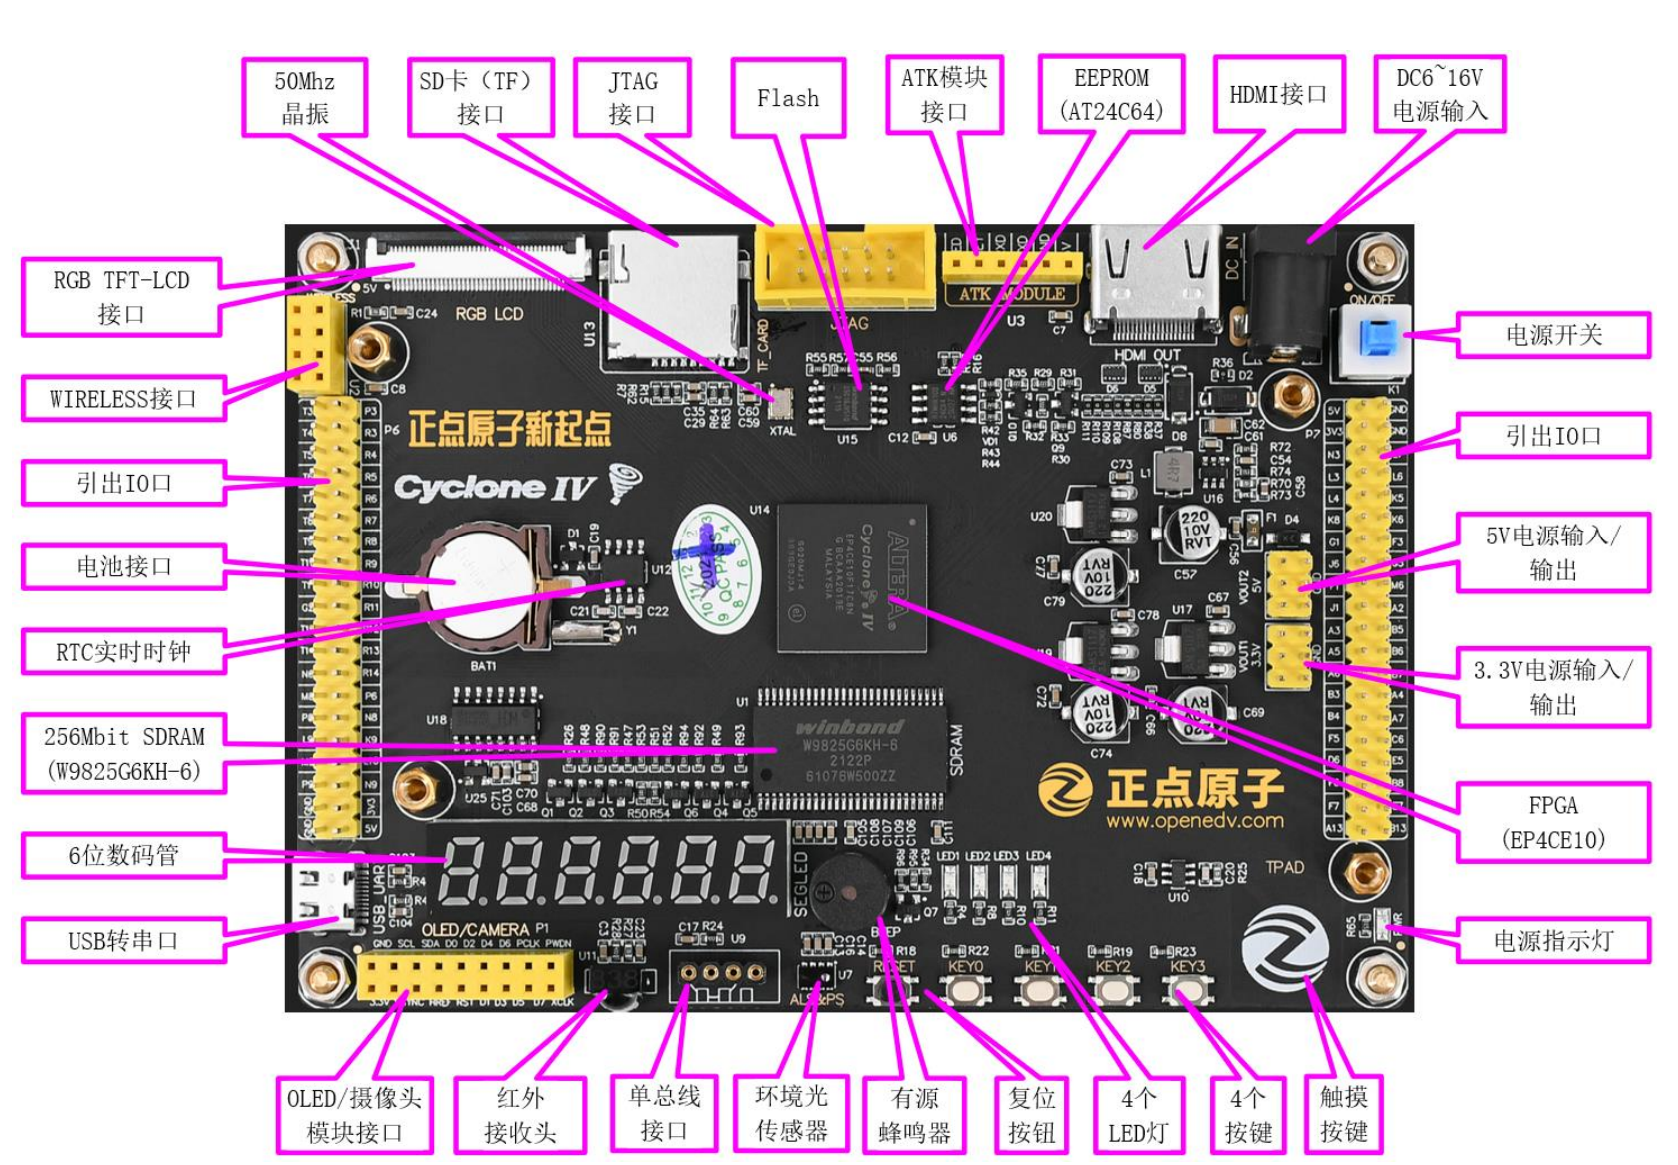
\includegraphics[width=0.8\textwidth]{FPGA.png}
    \caption{实验仪器与用具}
    \label{fig:实验仪器与用具}
\end{figure}

新起点 FPGA 开发板板载资源如下:

\begin{itemize}
    \item 主控芯片:EP4CE10F17C8N,封装:BGA256
    \item 晶振:50\,MHz
    \item FLASH:W25Q16,容量:16\,Mbit(2\,M字节)
    \item SDRAM:W9825G6KH-6,容量:256\,Mbit(32\,M字节)
    \item EEPROM:AT24C64,容量:64\,Kbit(8\,K字节)
    \item 1 个电源指示灯(蓝色)
    \item 4 个状态指示灯(DS0~DS3:红色)
    \item 1 个红外接收头,并配备一款小巧的红外遥控器
    \item 1 个无线模块接口,支持 NRF24L01 无线模块
    \item 1 路单总线接口,支持 DS18B20/DHT11 等单总线传感器
    \item 1 个 ATK 模块接口,支持正点原子蓝牙/GPS/MPU6050/RGB 灯模块
    \item 1 个环境光传感器,采用 AP3216C 芯片
    \item 1 个标准的 RGB TFT-LCD 接口
    \item 1 个 OLED/摄像头模块接口
    \item 1 个 USB 串口
    \item 1 个有源蜂鸣器
    \item 1 个 SD 卡接口(在板子背面)
    \item 1 个 HDMI 接口
    \item 1 个标准的 JTAG 调试下载口
    \item 1 组 5V 电源供应/接入口
    \item 1 组 3.3V 电源供应/接入口
    \item 1 个直流电源输入接口(输入电压范围:DC6~16V)
    \item 1 个 RTC 后备电池座,并带电池(在板子背面)
    \item 1 个 RTC 实时时钟,采用 PCF8563 芯片
    \item 1 个复位按钮,可作为 FPGA 程序执行的复位信号
    \item 4 个功能按钮
    \item 1 个电容触摸按键
    \item 1 个电源开关,控制整个开发板的电源
    \item 两个 20$\times$2 扩展口,共 72 个扩展 IO 口(除去电源和地)
\end{itemize}

\section{实验内容与步骤}
\subsection{概述}
\textbf{LED 流水灯实验:}
\begin{enumerate}
\item[A.] 按照指南开发指南第八章(P198)复现LED流水灯实验,仿真部分暂时不用做
\item[B.] 固化程序到开发板中,实现断开下载器、电源后重启仍可实现LED流水灯
\end{enumerate}

\textbf{按键控制 LED 灯实验:}
\begin{enumerate}
\item[A.] 按照指南开发指南第九章(P206)复现按键控制流水灯实验,仿真部分暂时不用做
\item[B.] 修改原实验的按键逻辑,使其分别实现下述功能:
\item 按键1,2,4保持原功能不变,按下按键3会使LED灯按照从左向右的顺序流水,时间间隔设置为1s
\item 按下对应按键,松开按钮LED也会保持按键对应的逻辑运行(用寄存器存储上一个按下的按钮状态)
\end{enumerate}

\subsection{实验步骤}

\begin{enumerate}
    \item 新建 Project
    \begin{figure}[H]
        \centering
        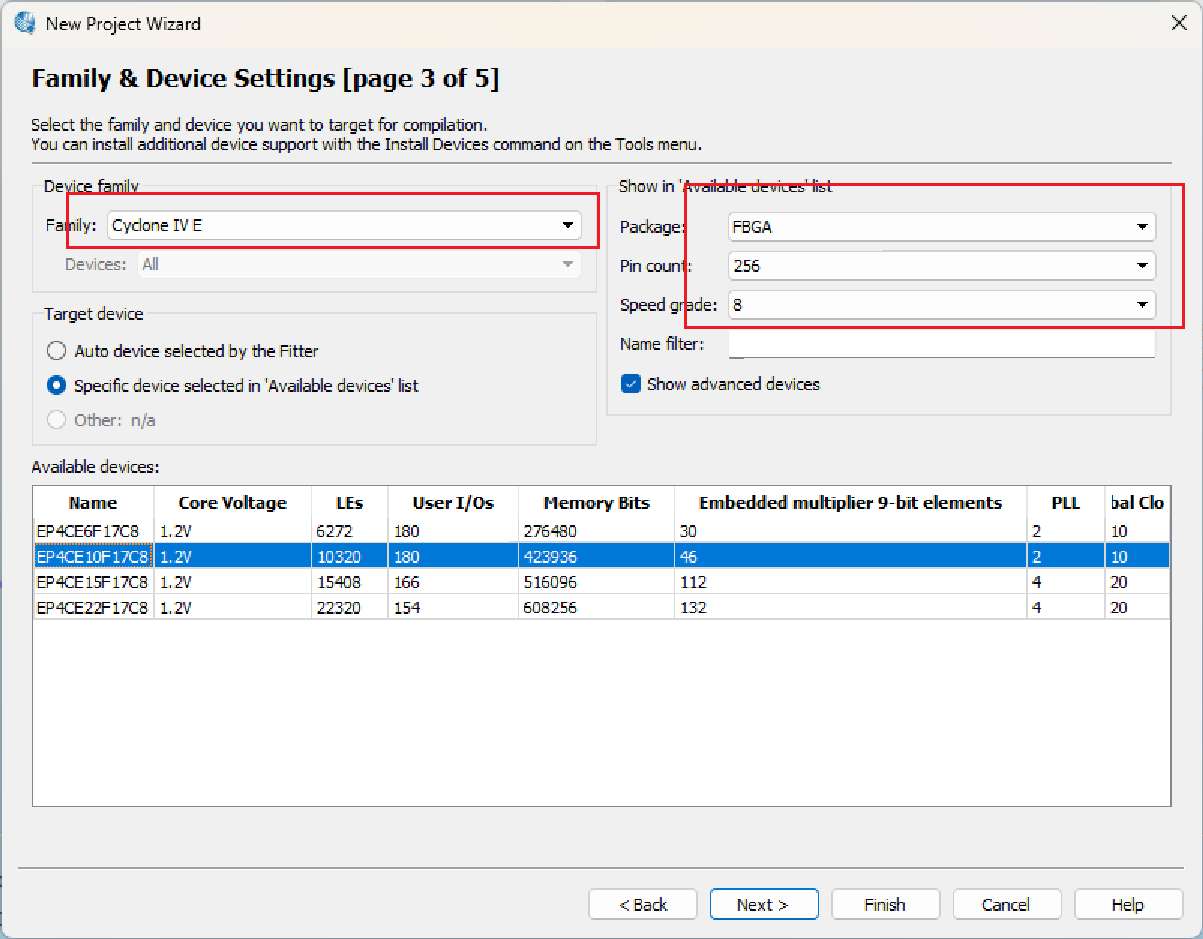
\includegraphics[width=0.7\textwidth]{step1.png}
        \caption{新建 Project 的操作界面}
        \label{fig:step1}
    \end{figure}
    \begin{figure}[H]
        \centering
        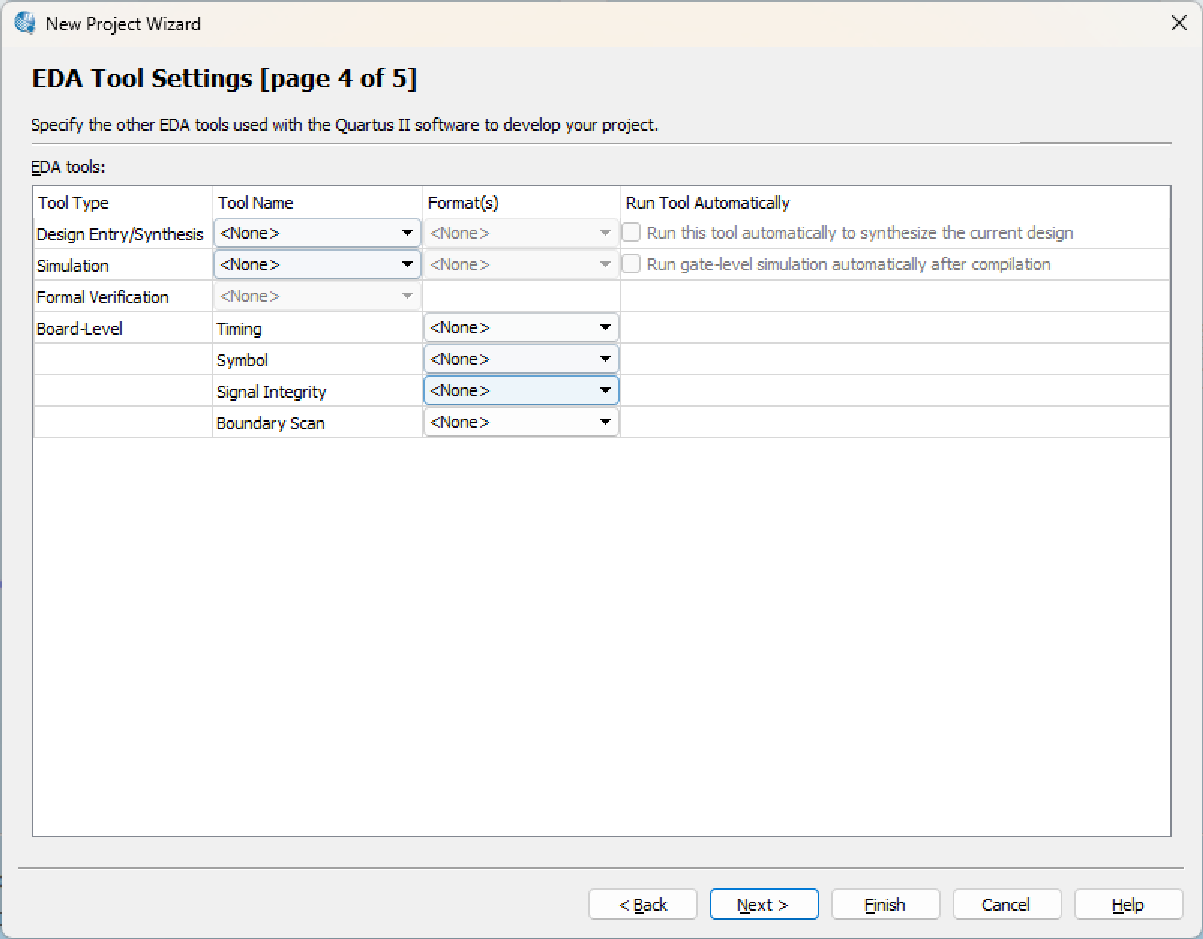
\includegraphics[width=0.7\textwidth]{step1_2.png}
        \caption{新建 Project 的操作界面}
        \label{fig:step1_2}
    \end{figure}
    \textbf{说明:}(此处填写新建工程的详细步骤和注意事项)

    \item 新建 .v 文件,编写代码并测试编译
    \begin{figure}[H]
        \centering
        \begin{subfigure}{0.3\textwidth}
            \centering
            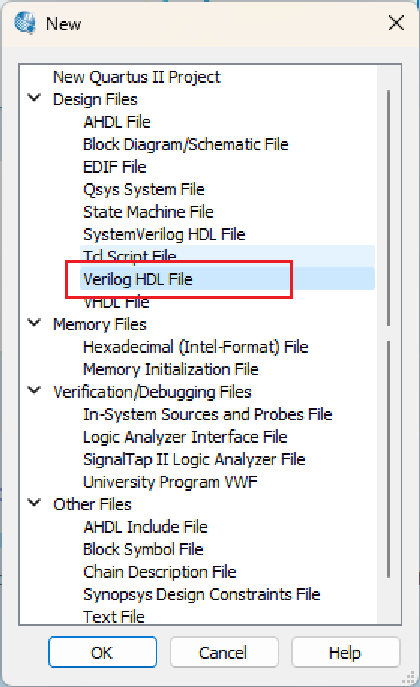
\includegraphics[width=\linewidth]{step2.png}
            \caption{新建 Verilog 文件}
            \label{fig:step2}
        \end{subfigure}
        \hfill
        \begin{subfigure}{0.68\textwidth}
            \centering
            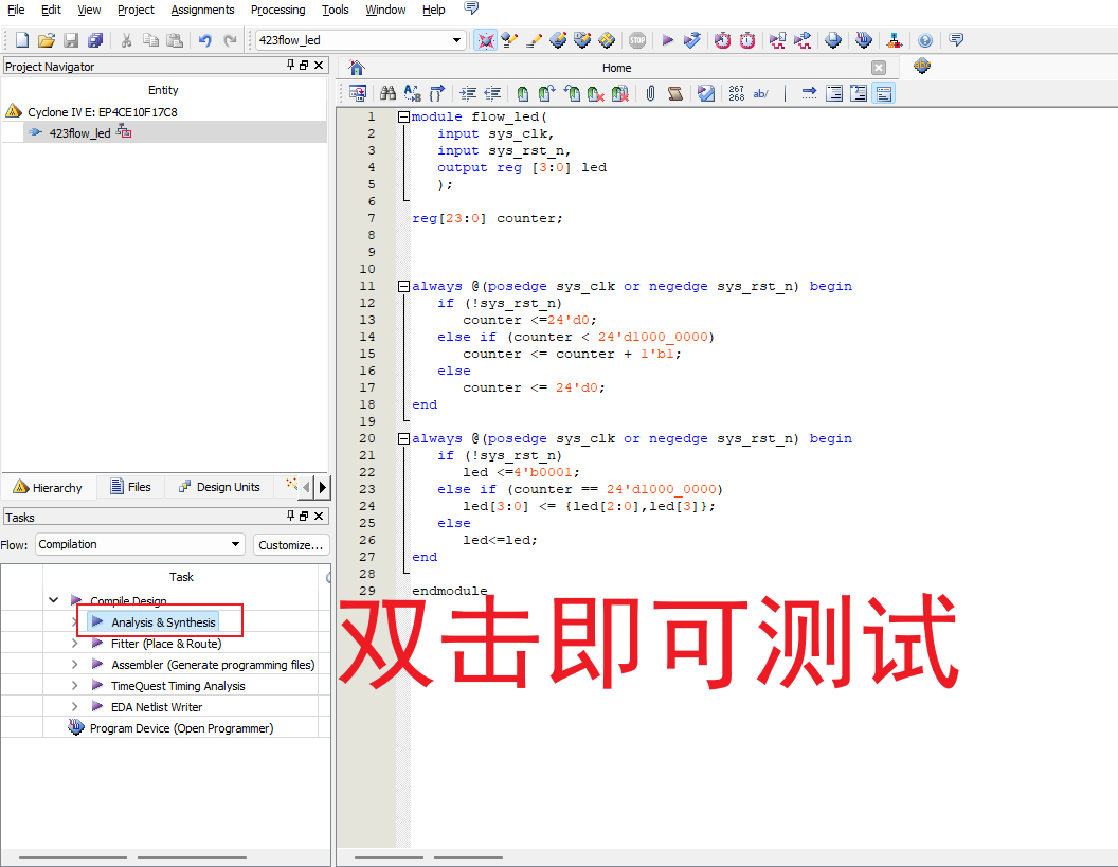
\includegraphics[width=\linewidth]{step2_2.png}
            \caption{代码编写界面}
            \label{fig:step2_2}
        \end{subfigure}
    \end{figure}
    \textbf{说明:}(此处填写代码编写、保存及测试编译的详细说明)
    
\cleardoublepage
    \item 预编译,确认无误
    \begin{figure}[H]
        \centering
        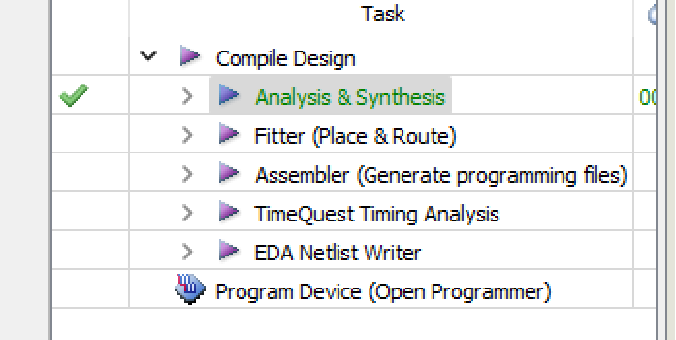
\includegraphics[width=0.7\textwidth]{step3.png}
        \caption{预编译结果界面1}
        \label{fig:step3}
    \end{figure}
    \begin{figure}[H]
        \centering
        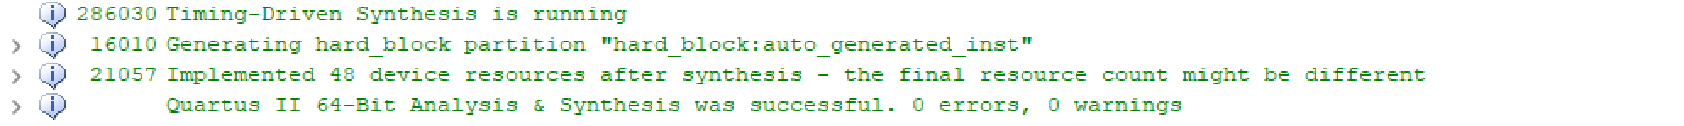
\includegraphics[width=0.7\textwidth]{step3_2.png}
        \caption{预编译结果界面2}
        \label{fig:step3_2}
    \end{figure}
    \textbf{说明:}(此处填写预编译通过的判断方法及常见问题)

\vspace{1cm}
    
    \item 注意 Project Name 和代码中的 module 名称一致
    \begin{figure}[H]
        \centering
        \begin{subfigure}{0.5\textwidth}
            \centering
            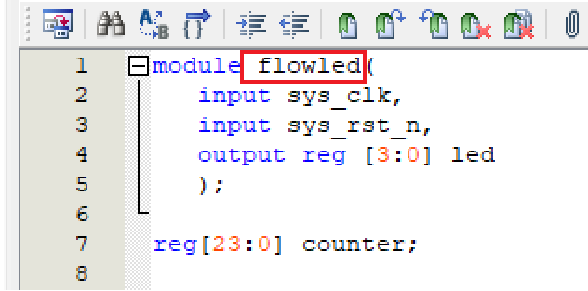
\includegraphics[width=\linewidth]{step4.png}
            \caption{Project Name}
            \label{fig:step4}
        \end{subfigure}
        \hfill
        \begin{subfigure}{0.45\textwidth}
            \centering
            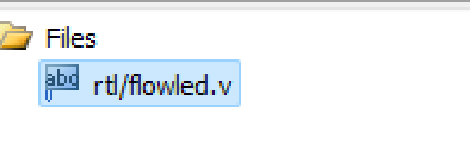
\includegraphics[width=\linewidth]{step4_2.png}
            \caption{module 名称}
            \label{fig:step4_2}
        \end{subfigure}
    \end{figure}
    \textbf{说明:}(此处说明为何需要一致及如何检查)

\cleardoublepage
    \item 保存代码文件至 rtl 文件夹内
    \begin{figure}[H]
        \centering
        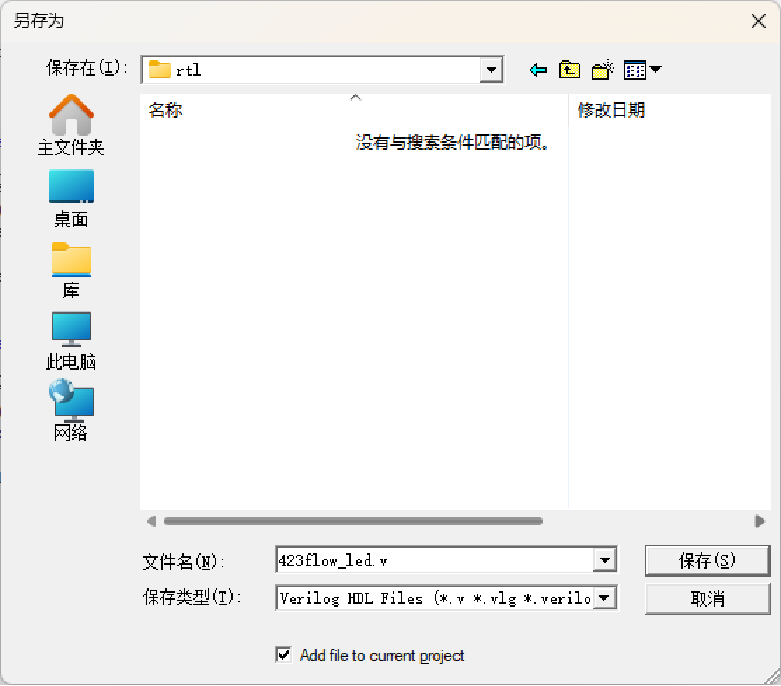
\includegraphics[width=0.7\textwidth]{step5.png}
        \caption{保存代码文件到指定文件夹}
        \label{fig:step5}
    \end{figure}
    \textbf{说明:}(此处说明文件管理规范)

    \item 打开 Pin Planner 分配引脚
    \begin{figure}[H]
        \centering
        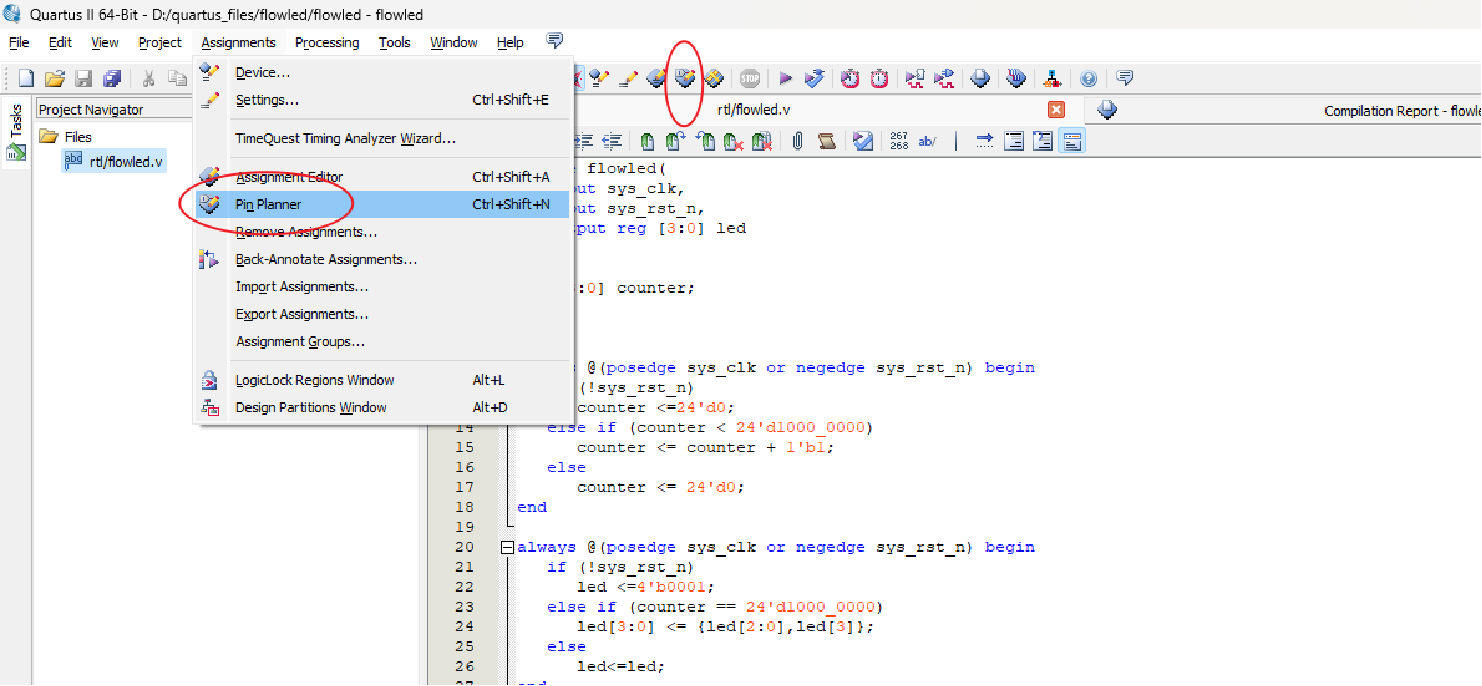
\includegraphics[width=0.8\textwidth]{step6.png}
        \caption{Pin Planner 分配引脚界面}
        \label{fig:step6}
    \end{figure}
    \textbf{说明:}(此处填写分配引脚的详细步骤)

\cleardoublepage

    \item 手动输入/使用 tcl 脚本文件
    \begin{figure}[H]
        \centering
        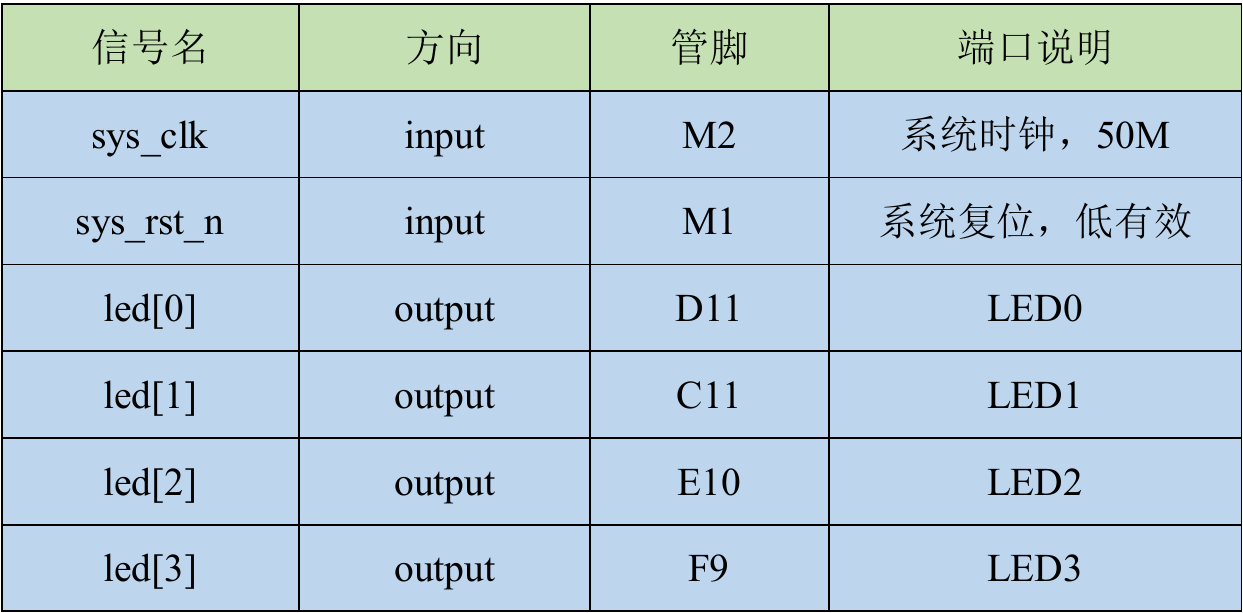
\includegraphics[width=0.7\textwidth]{step7.png}
        \caption{tcl 脚本分配引脚示意}
        \label{fig:step7}
    \end{figure}
    \textbf{tcl 脚本示例:}
    \begin{lstlisting}[language=Matlab, style=MatlabStyle_src]
        set_location_assignment PIN_M2 -to sys_clk
        set_location_assignment PIN_M1 -to sys_rst_n
        set_location_assignment PIN_D11 -to led[0]
        set_location_assignment PIN_C11 -to led[1]
        set_location_assignment PIN_E10 -to led[2]
        set_location_assignment PIN_F9 -to led[3]
    \end{lstlisting}
    \textbf{说明:}(此处说明两种方式的区别和操作方法)

    \item 完整编译工程
    \begin{figure}[H]
        \centering
        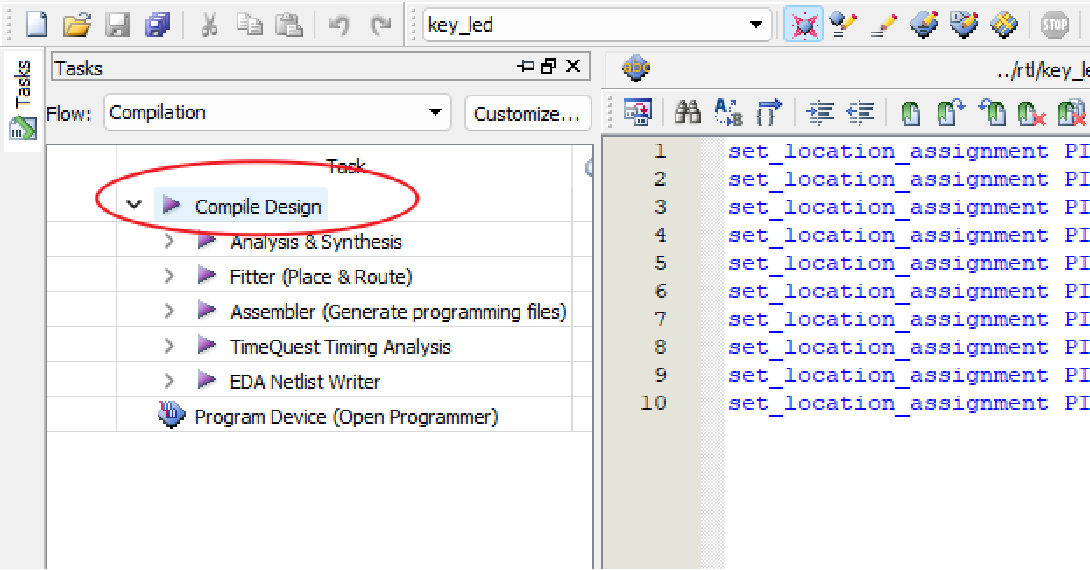
\includegraphics[width=0.7\textwidth]{step8.png}
        \caption{完整编译工程界面}
        \label{fig:step8}
    \end{figure}
    \textbf{说明:}(此处填写完整编译的流程和注意事项)

\cleardoublepage

    \item 下载程序至开发板
    \begin{figure}[H]
        \centering
        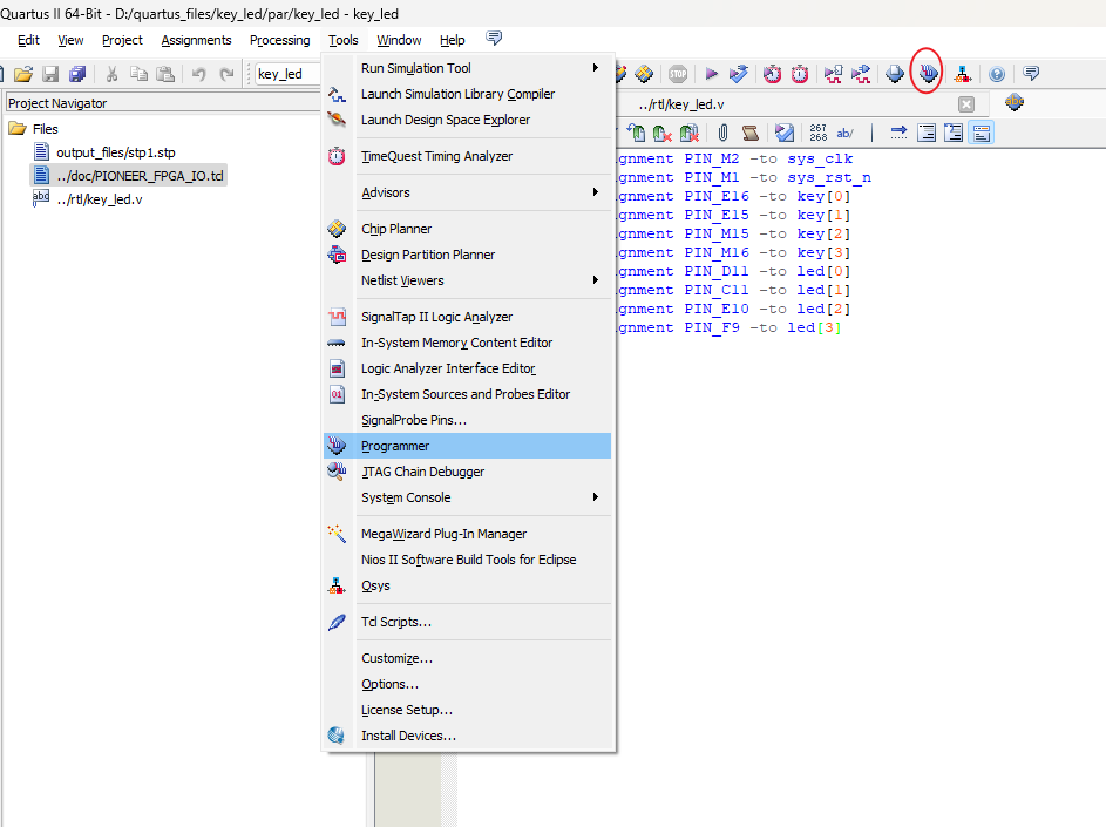
\includegraphics[width=0.7\textwidth]{step9.png}
        \caption{下载程序到开发板界面1}
        \label{fig:step9}
    \end{figure}

    \begin{figure}[H]
        \centering
        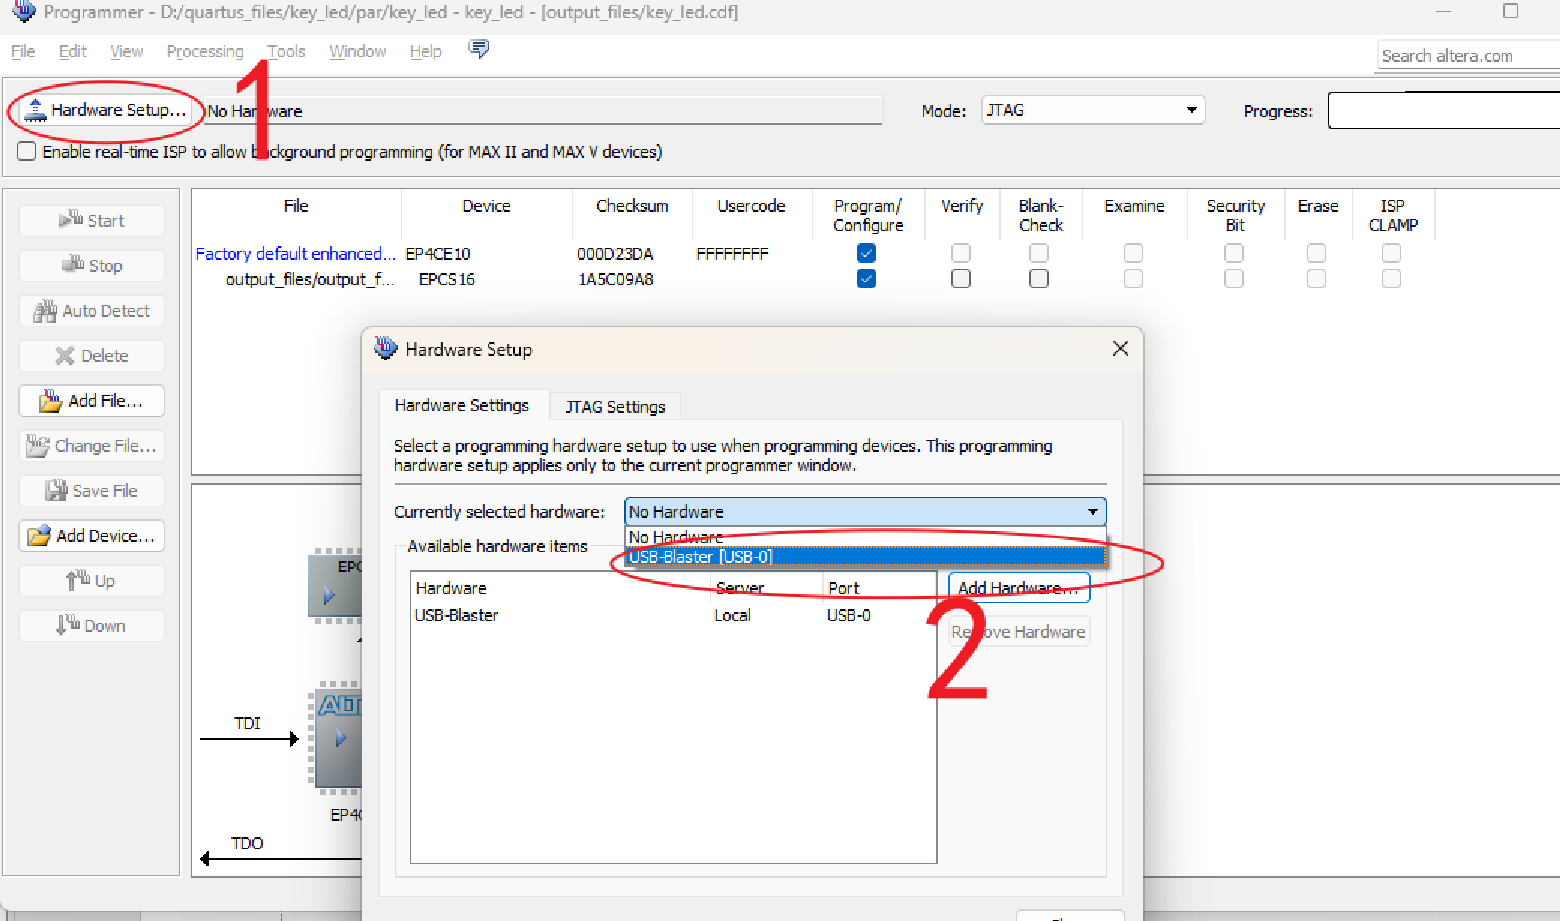
\includegraphics[width=0.7\textwidth]{step9_2.png}
        \caption{下载程序到开发板界面2}
        \label{fig:step9_2}
    \end{figure}

    \begin{figure}[H]
        \centering
        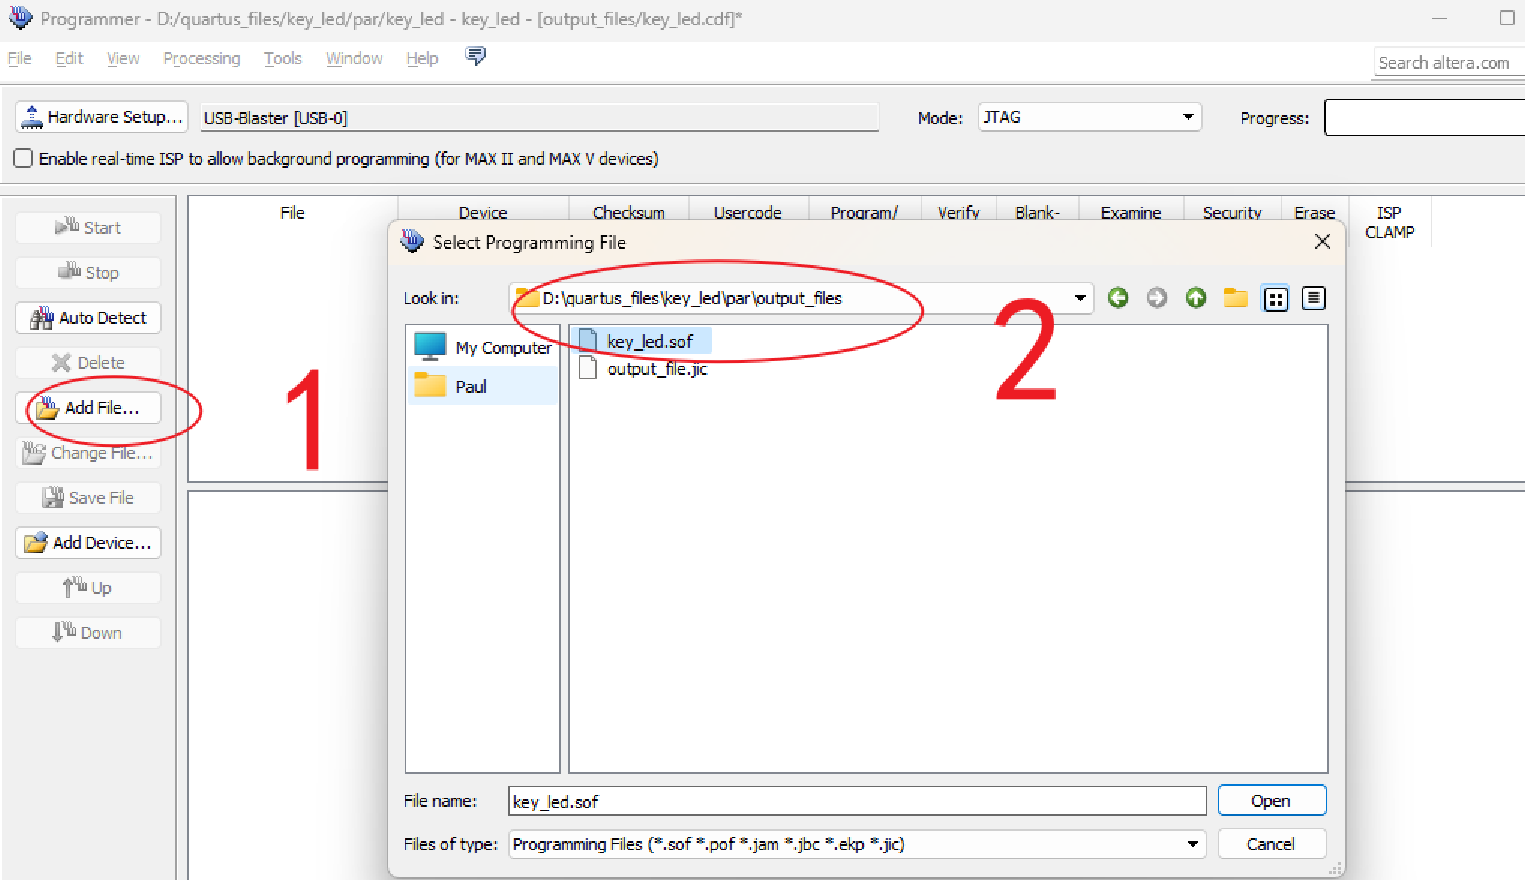
\includegraphics[width=0.7\textwidth]{step9_3.png}
        \caption{下载程序到开发板界面3}
        \label{fig:step9_3}
    \end{figure}

    \begin{figure}[H]
        \centering
        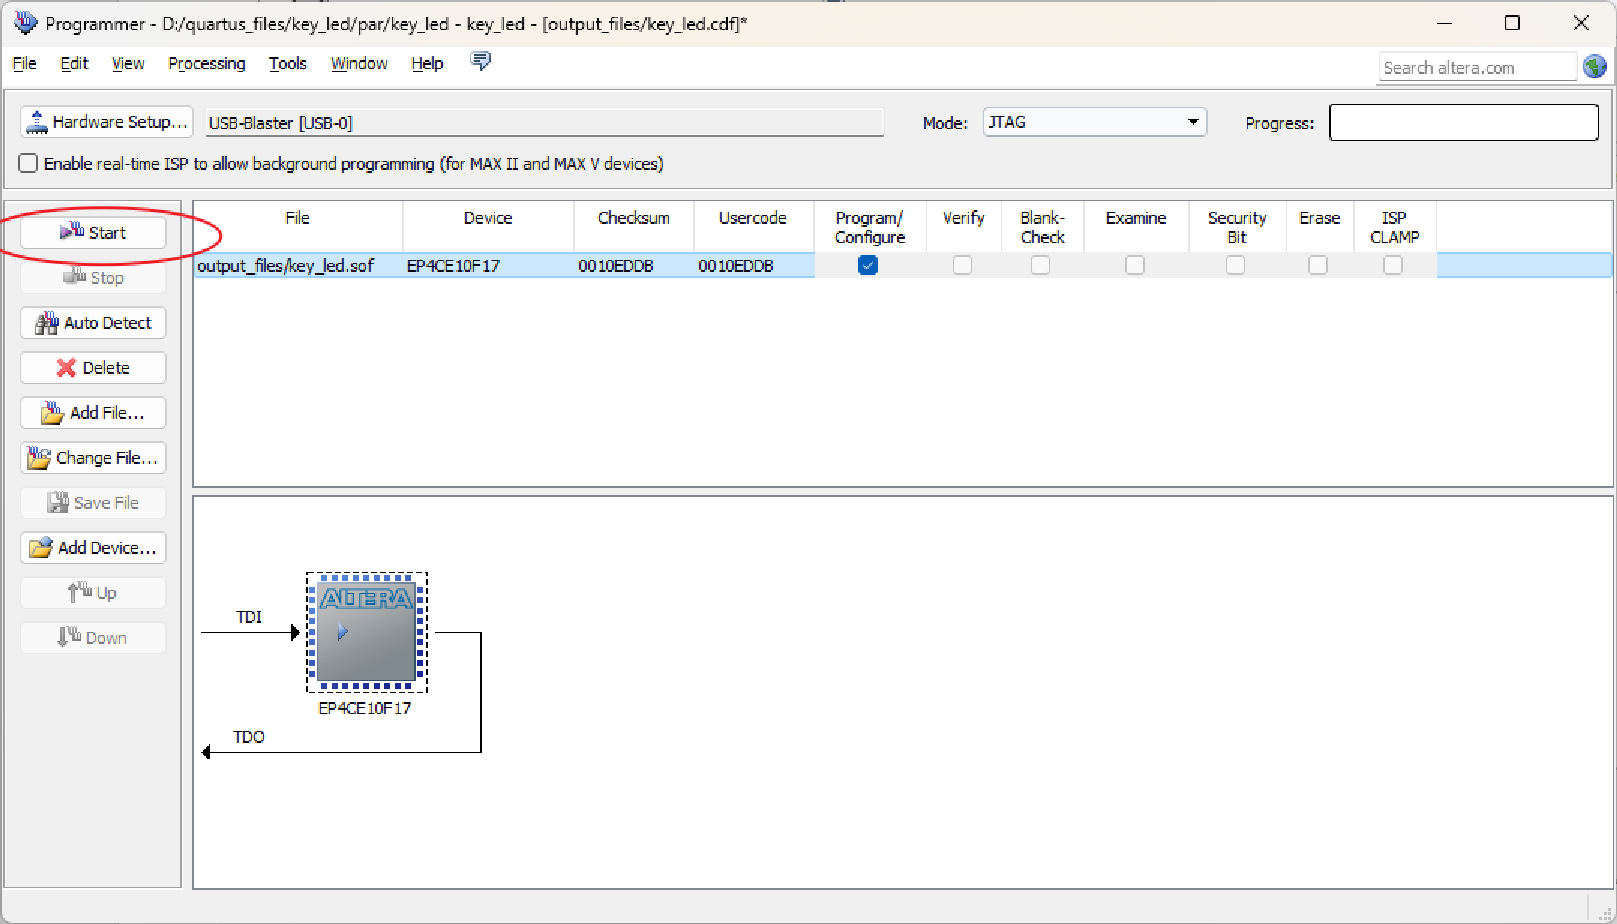
\includegraphics[width=0.7\textwidth]{step9_4.png}
        \caption{下载程序到开发板界面4}
        \label{fig:step9_4}
    \end{figure}
    \textbf{说明:}(此处填写下载步骤和常见问题)

    \item 导出 jic 文件,固化程序
    \begin{figure}[H]
        \centering
        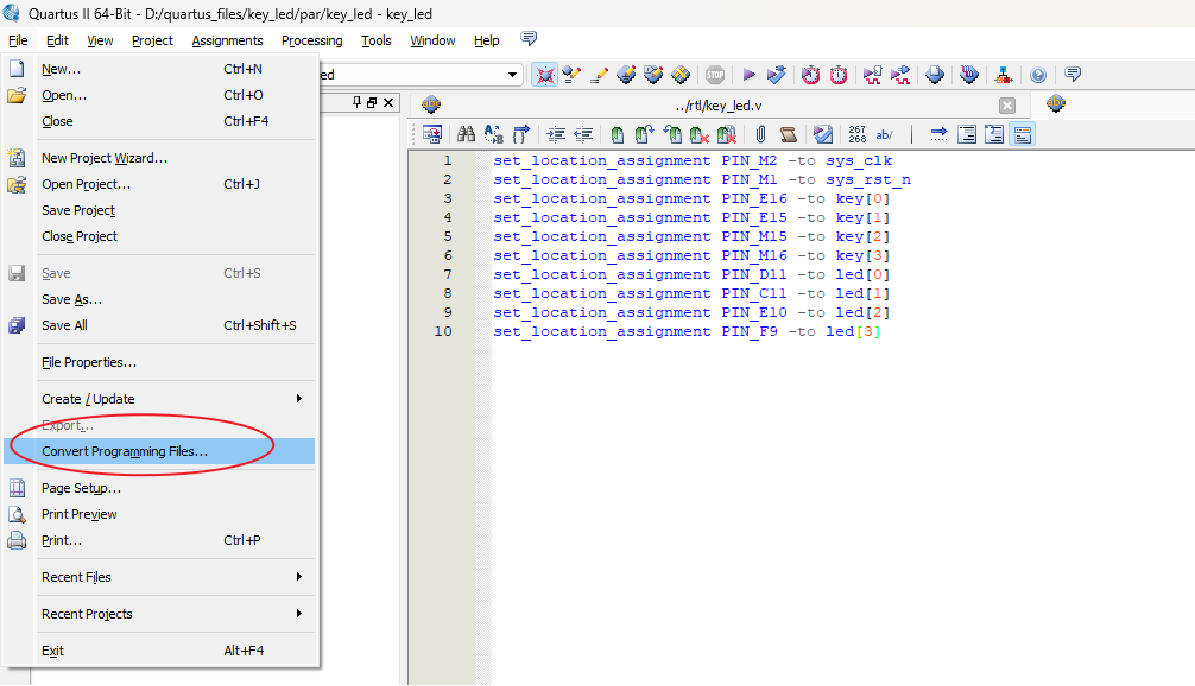
\includegraphics[width=0.7\textwidth]{step10.png}
        \caption{导出 jic 文件界面}
        \label{fig:step10}
    \end{figure}

    \begin{figure}[H]
        \centering
        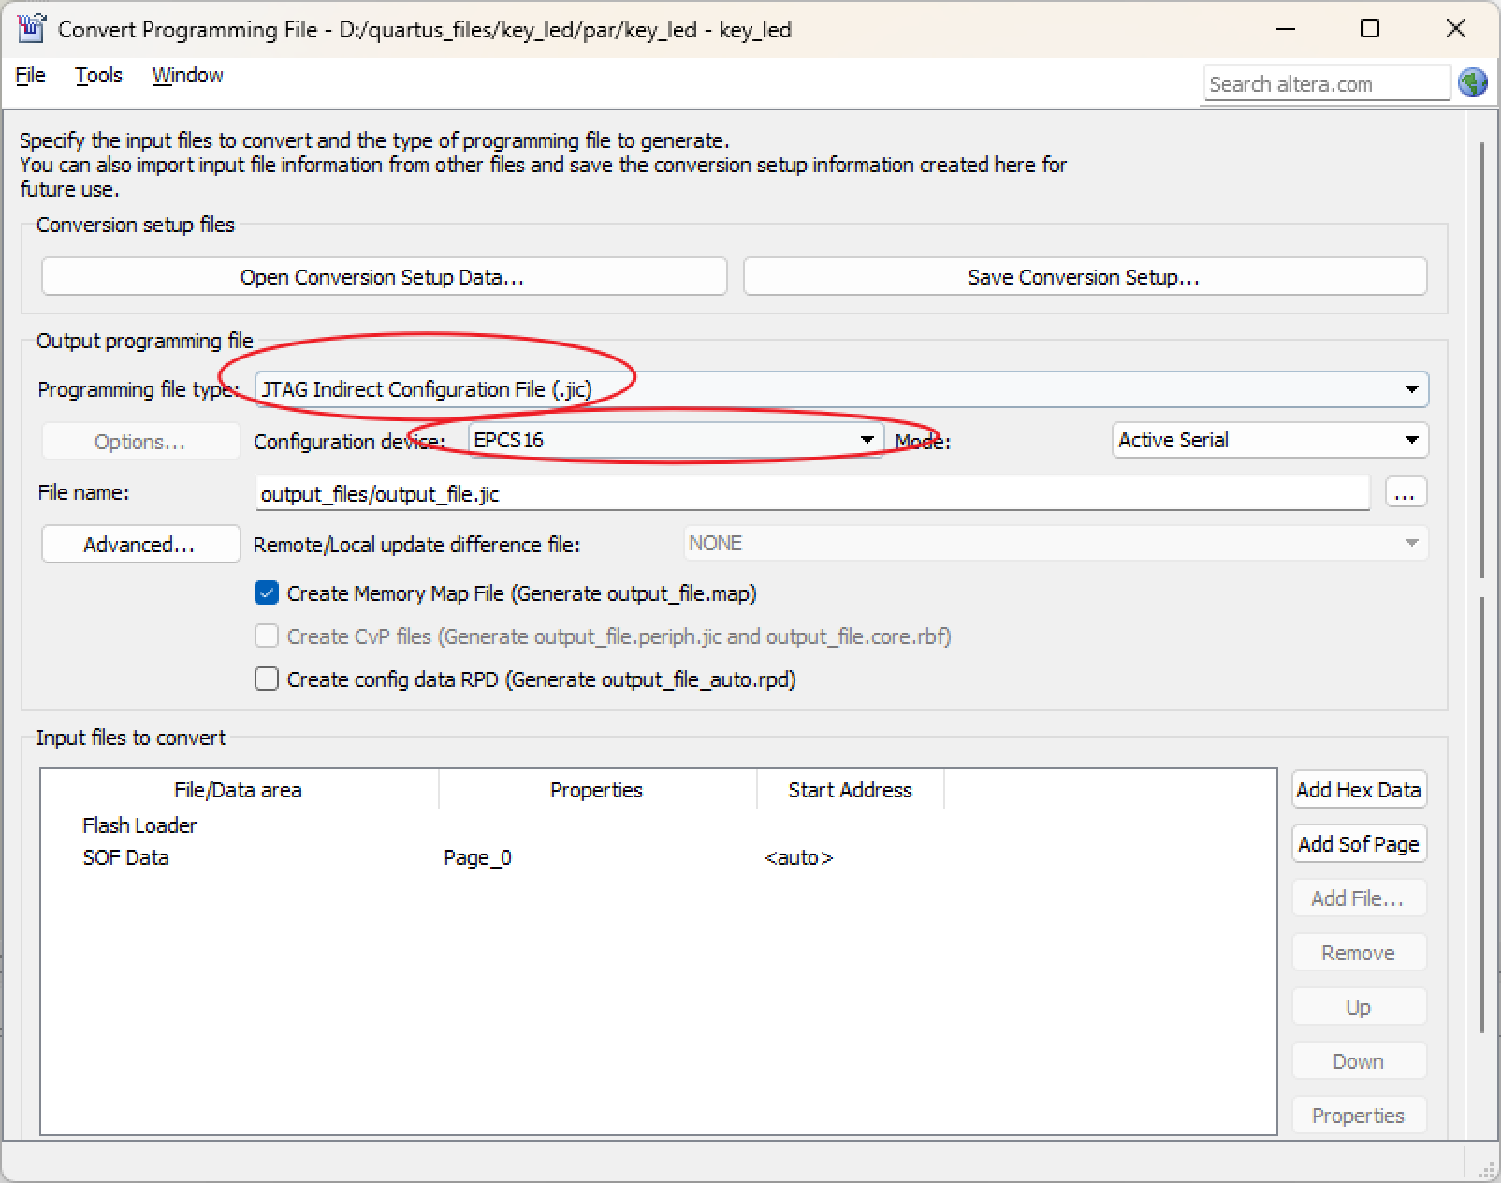
\includegraphics[width=0.7\textwidth]{step10_2.png}
        \caption{导出 jic 文件界面2}
        \label{fig:step10_2}
    \end{figure}

    \begin{figure}[H]
        \centering
        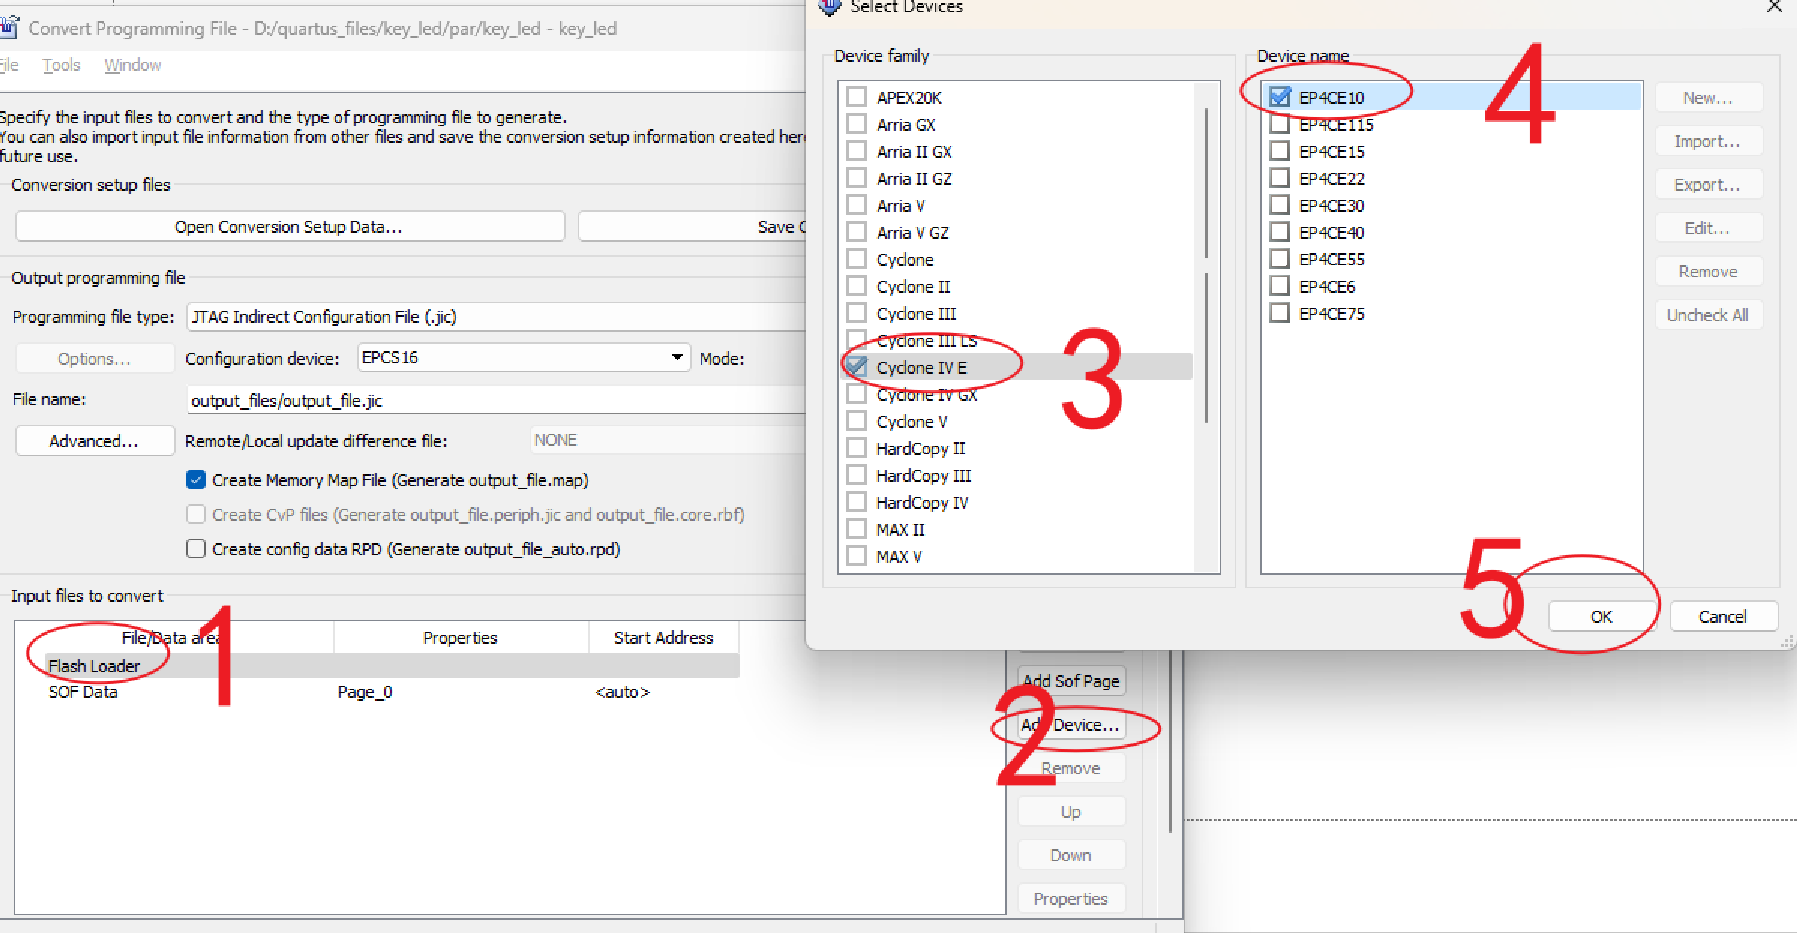
\includegraphics[width=0.7\textwidth]{step10_3.png}
        \caption{导出 jic 文件界面3}
        \label{fig:step10_3}
    \end{figure}

    \begin{figure}[H]
        \centering
        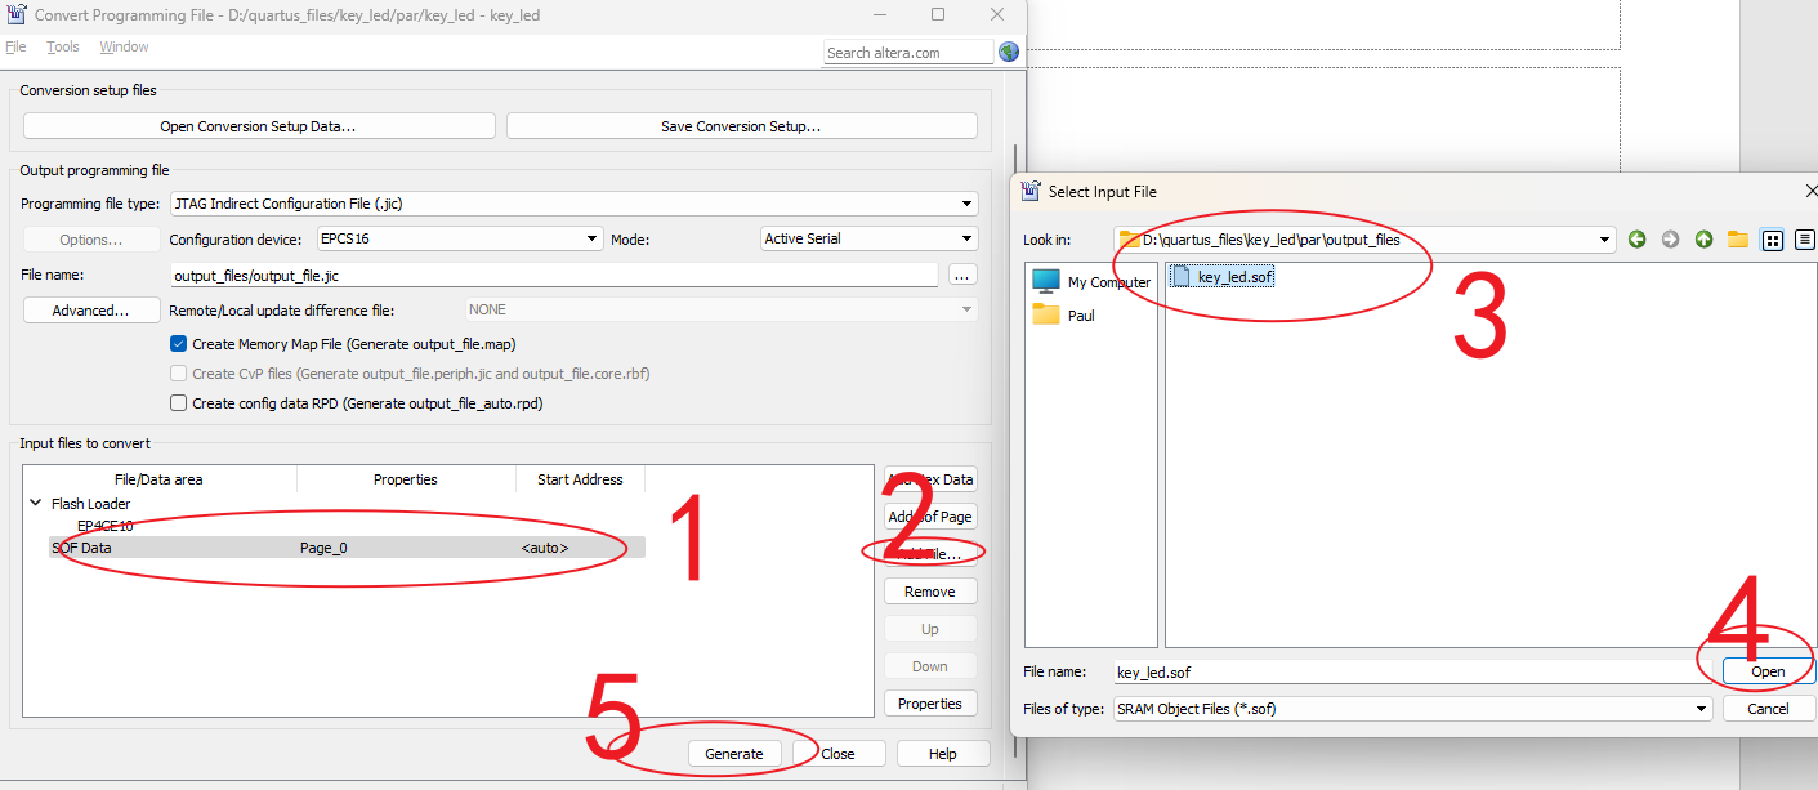
\includegraphics[width=0.7\textwidth]{step10_4.png}
        \caption{导出 jic 文件界面4}
        \label{fig:step10_4}
    \end{figure}

    \textbf{说明:}(此处填写固化流程和注意事项)
\end{enumerate}




\cleardoublepage

\section{实验结果}

\subsection{实验结果1:LED 流水灯实验}
\noindent
\textbf{演示视频:}\href{https://www.bilibili.com/video/BV1H1VtzYEMq/?share_source=copy_web&vd_source=4fd6c4265e65c0785c912874692a3971}{点击查看演示视频}

\subsection{实验结果2:按键控制 LED 灯实验基础问题}
\noindent
\textbf{演示视频:}\href{https://www.bilibili.com/video/BV1c1VtzYEpA/?share_source=copy_web&vd_source=4fd6c4265e65c0785c912874692a3971}{点击查看演示视频}

\subsection{实验结果3:按键控制 LED 灯实验变式1}
\noindent
\textbf{演示视频:}\href{https://www.bilibili.com/video/BV1AyVtzPEPV/?share_source=copy_web&vd_source=4fd6c4265e65c0785c912874692a3971}{点击查看演示视频}

\subsection{实验结果4:按键控制 LED 灯实验变式2}
\noindent
\textbf{演示视频:}\href{https://www.bilibili.com/video/BV1wyVtzPE7z/?share_source=copy_web&vd_source=4fd6c4265e65c0785c912874692a3971}{点击查看演示视频}



\section{实验总结}

\subsection{实验中的问题与感想}

\begin{enumerate}
    \item 在实验过程中,遇到了一些问题,例如:编译错误、引脚分配不当等。通过查阅资料和请教老师,最终解决了这些问题。
    \item 通过本次实验,我对 FPGA 开发流程有了更深入的理解,尤其是在代码编写和调试方面。
    \item 实验中使用的 Verilog 语言让我对硬件描述语言有了更直观的认识,增强了我的编程能力。
    \item 通过对 LED 流水灯和按键控制 LED 灯的实验,我对数字电路的基本原理有了更深入的理解。
    \item 在实验中,我还学会了如何使用 Quartus 软件进行 FPGA 开发和调试,这对我今后的学习和工作都非常有帮助。
\end{enumerate}

\cleardoublepage
\section{附录:Verilog 代码}

\textbf{Verilog 代码:LED 流水灯实验}
\begin{lstlisting}[language=Matlab, style=MatlabStyle_src]
module flow_led(
	input sys_clk,
	input sys_rst_n,
	output reg [3:0] led
	);
	
reg [23:0] counter;

always @(posedge sys_clk or negedge sys_rst_n) begin
	if (!sys_rst_n)
		counter <= 24'd0;
	else if (counter < 24'd1000_0000)
		counter <= counter + 1'b1;
	else
		counter <= 24'd0;
end


always @(posedge sys_clk or negedge sys_rst_n) begin
	if (!sys_rst_n)
		led <= 4'b0001;
	else if(counter == 24'd1000_0000)
		led[3:0] <= {led[2:0],led[3]};
	else
		led <= led;
end

endmodule

\end{lstlisting}

\cleardoublepage

\textbf{Verilog 代码:按键控制 LED 灯实验基础}
\begin{lstlisting}[language=Matlab, style=MatlabStyle_src]
    module key_led(
        input sys_clk,
        input sys_rst_n,
        input [3:0] key,
        output reg [3:0] led
        );
        
        
    reg [23:0] cnt;
    reg [1:0] led_control;
    
    always @ (posedge sys_clk or negedge sys_rst_n) begin
        if (!sys_rst_n)
            cnt<=24'd9_999_999;
        else if(cnt<24'd9_999_999)
            cnt<=cnt+1;
        else
            cnt<=0;
    end
    
    
    always @ (posedge sys_clk or negedge sys_rst_n) begin
        if (!sys_rst_n)
            led_control <= 2'b00;
        else if(cnt == 24'd9_999_999)
            led_control <= led_control + 1'b1;
        else
            led_control <= led_control;
    end
    
    
    always @ (posedge sys_clk or negedge sys_rst_n) begin
        if (!sys_rst_n) begin
            led <= 4'b 0000;
        end
        else if (key[0]==0)
            case (led_control)
                2'b00 : led<=4'b1000;
                2'b01 : led<=4'b0100;
                2'b10 : led<=4'b0010;
                2'b11 : led<=4'b0001;
                default : led<=4'b0000;
            endcase
        else if (key[1]==0)
            case (led_control)
                2'b00 : led<=4'b0001;
                2'b01 : led<=4'b0010;
                2'b10 : led<=4'b0100;
                2'b11 : led<=4'b1000;
                default : led<=4'b0000;
            endcase
        else if (key[2]==0)
            case (led_control)
                2'b00 : led <=4'b1111;
                2'b01 : led <=4'b0000;
                2'b10 : led <=4'b1111;
                2'b11 : led <=4'b0000;
                default : led <=4'b0000;
            endcase
        else if (key[3]==0)
                led<=4'b1111;
        else
            led<=4'b0000;
    end 
    
    endmodule
                
\end{lstlisting}


\cleardoublepage

\textbf{Verilog 代码:按键控制 LED 灯实验变式1}
\begin{lstlisting}[language=Matlab, style=MatlabStyle_src]
module key_leda(
    input sys_clk,
    input sys_rst_n,
    input [3:0] key,
    output reg [3:0] led
);

reg [23:0] cnt;
reg [25:0] cnt_1s;  // New counter for 1-second interval
reg [1:0] led_control;
reg [1:0] flow_control;  // New control for flowing sequence

// Counter for 0.2-second interval (original timing)
always @ (posedge sys_clk or negedge sys_rst_n) begin
    if (!sys_rst_n)
        cnt <= 24'd9_999_999;
    else if (cnt < 24'd9_999_999)
        cnt <= cnt + 1;
    else
        cnt <= 0;
end

// Counter for 1-second interval (for key[2])
always @ (posedge sys_clk or negedge sys_rst_n) begin
    if (!sys_rst_n)
        cnt_1s <= 26'd0;
    else if (cnt_1s < 26'd49_999_999)
        cnt_1s <= cnt_1s + 1;
    else
        cnt_1s <= 0;
end

// led_control increments every 0.2 seconds
always @ (posedge sys_clk or negedge sys_rst_n) begin
    if (!sys_rst_n)
        led_control <= 2'b00;
    else if (cnt == 24'd9_999_999)
        led_control <= led_control + 1'b1;
    else
        led_control <= led_control;
end

// flow_control increments every 1 second
always @ (posedge sys_clk or negedge sys_rst_n) begin
    if (!sys_rst_n)
        flow_control <= 2'b00;
    else if (cnt_1s == 26'd49_999_999)
        flow_control <= flow_control + 1'b1;
    else
        flow_control <= flow_control;
end

// LED control logic
always @ (posedge sys_clk or negedge sys_rst_n) begin
    if (!sys_rst_n) begin
        led <= 4'b0000;
    end
    else if (key[0] == 0)  // Original function: shift right every 0.2s
        case (led_control)
            2'b00 : led <= 4'b1000;
            2'b01 : led <= 4'b0100;
            2'b10 : led <= 4'b0010;
            2'b11 : led <= 4'b0001;
            default : led <= 4'b0000;
        endcase
    else if (key[1] == 0)  // Original function: shift left every 0.2s
        case (led_control)
            2'b00 : led <= 4'b0001;
            2'b01 : led <= 4'b0010;
            2'b10 : led <= 4'b0100;
            2'b11 : led <= 4'b1000;
            default : led <= 4'b0000;
        endcase
    else if (key[2] == 0)  // Modified function: flow left to right every 1s
        case (flow_control)
            2'b00 : led <= 4'b1000;
            2'b01 : led <= 4'b0100;
            2'b10 : led <= 4'b0010;
            2'b11 : led <= 4'b0001;
            default : led <= 4'b0000;
        endcase
    else if (key[3] == 0)  // Original function: all LEDs on
        led <= 4'b1111;
    else
        led <= 4'b0000;
end

endmodule
\end{lstlisting}

\cleardoublepage

\textbf{Verilog 代码:按键控制 LED 灯实验变式2}
\begin{lstlisting}[language=Matlab, style=MatlabStyle_src]
    module key_ledb(
        input sys_clk,
        input sys_rst_n,
        input [3:0] key,
        output reg [3:0] led
        );
        
    reg [23:0] cnt;
    reg [1:0] led_control;
    reg [1:0] mode;
    reg active;
    
    // Counter logic: counts up to 9,999,999 for timing
    always @ (posedge sys_clk or negedge sys_rst_n) begin
        if (!sys_rst_n)
            cnt <= 24'd0;  // Initialize to 0 for standard counter behavior
        else if (cnt < 24'd9_999_999)
            cnt <= cnt + 1;
        else
            cnt <= 0;
    end
    
    // LED control logic: increments every time cnt reaches 9,999,999
    always @ (posedge sys_clk or negedge sys_rst_n) begin
        if (!sys_rst_n)
            led_control <= 2'b00;
        else if (cnt == 24'd9_999_999)
            led_control <= led_control + 1'b1;
        else
            led_control <= led_control;
    end
    
    // Mode and active logic: stores the last pressed key and activates the pattern
    always @ (posedge sys_clk or negedge sys_rst_n) begin
        if (!sys_rst_n) begin
            mode <= 2'b00;  // Initial mode (arbitrary)
            active <= 0;    // Inactive until a key is pressed
        end
        else if (key[0] == 0) begin
            mode <= 2'b00;  // Key[0] pressed
            active <= 1;    // Activate pattern
        end
        else if (key[1] == 0) begin
            mode <= 2'b01;  // Key[1] pressed
            active <= 1;
        end
        else if (key[2] == 0) begin
            mode <= 2'b10;  // Key[2] pressed
            active <= 1;
        end
        else if (key[3] == 0) begin
            mode <= 2'b11;  // Key[3] pressed
            active <= 1;
        end
        else begin
            mode <= mode;   // Retain last mode
            active <= active; // Retain active state
        end
    end
    
    // LED output logic: sets LED pattern based on mode when active
    always @ (posedge sys_clk or negedge sys_rst_n) begin
        if (!sys_rst_n) begin
            led <= 4'b0000; // Reset LEDs to off
        end
        else if (active) begin
            case (mode)
                2'b00: begin // Key[0] pattern
                    case (led_control)
                        2'b00 : led <= 4'b1000;
                        2'b01 : led <= 4'b0100;
                        2'b10 : led <= 4'b0010;
                        2'b11 : led <= 4'b0001;
                    endcase
                end
                2'b01: begin // Key[1] pattern
                    case (led_control)
                        2'b00 : led <= 4'b0001;
                        2'b01 : led <= 4'b0010;
                        2'b10 : led <= 4'b0100;
                        2'b11 : led <= 4'b1000;
                    endcase
                end
                2'b10: begin // Key[2] pattern
                    case (led_control)
                        2'b00 : led <= 4'b1111;
                        2'b01 : led <= 4'b0000;
                        2'b10 : led <= 4'b1111;
                        2'b11 : led <= 4'b0000;
                    endcase
                end
                2'b11: begin // Key[3] pattern
                    led <= 4'b1111;
                end
            endcase
        end
        else begin
            led <= 4'b0000; // LEDs off when no key has been pressed
        end
    end
    
    endmodule
\end{lstlisting}




\end{document}

% VScode 常用快捷键:

% F2:                       变量重命名
% Ctrl + Enter:             行中换行
% Alt + up/down:            上下移行
% 鼠标中键 + 移动:           快速多光标
% Shift + Alt + up/down:    上下复制
% Ctrl + left/right:        左右跳单词
% Ctrl + Backspace/Delete:  左右删单词    
% Shift + Delete:           删除此行
% Ctrl + J:                 打开 VScode 下栏(输出栏)
% Ctrl + B:                 打开 VScode 左栏(目录栏)
% Ctrl + `:                 打开 VScode 终端栏
% Ctrl + 0:                 定位文件
% Ctrl + Tab:               切换已打开的文件(切标签)
% Ctrl + Shift + P:         打开全局命令(设置)

% Latex 常用快捷键:

% Ctrl + Alt + J:           由代码定位到PDF
% Ctrl + S:                 保存